\documentclass{article} % For LaTeX2e
\usepackage{iclr2027_conference,times}

% Uncomment for the camera-ready version, but NOT for submission.
% \iclrfinalcopy

% if you need to pass options to natbib, use, e.g.:
%     \PassOptionsToPackage{numbers, compress}{natbib}
% before loading iclr2027_conference

\usepackage[utf8]{inputenc} % allow utf-8 input
\usepackage[T1]{fontenc}    % use 8-bit T1 fonts
\usepackage{hyperref}       % hyperlinks
\usepackage{url}            % simple URL typesetting
\usepackage{booktabs}       % professional-quality tables
\usepackage{amsfonts}       % blackboard math symbols
\usepackage{amsmath}
\usepackage{amssymb}
\usepackage{nicefrac}       % compact symbols for 1/2, etc.
\usepackage{microtype}      % microtypography
\usepackage{xcolor}         % colors
\usepackage{graphicx}
\usepackage{caption}
\usepackage{subcaption}
\usepackage{float}
\usepackage{afterpage}
\usepackage{paralist}

% ──────────────────────────── Algorithm pseudo-code ───────────────────────
% Pseudo-code helpers (works in regular text)
\newcommand{\kwFor}[1]{\textbf{for} #1 \textbf{do}}
\newcommand{\kwIf}[1]{\textbf{if} #1 \textbf{then}}
\newcommand{\kwElse}{\textbf{else}}
\newcommand{\kwEnd}[1]{\textbf{end} \textbf{#1}}
\newcommand{\kwReturn}{\textbf{return}~}
\newcommand{\kwRequire}{\textbf{Input:}~}
\newcommand{\kwEnsure}{\textbf{Output:}~}
\newcommand{\Comment}[1]{\hfill{\color{gray}\textit{// #1}}}
\newcommand{\Lstate}[1]{\par\hangindent=1em\noindent\hspace{1em}#1}
\newcommand{\LstateII}[1]{\par\hangindent=2em\noindent\hspace{2em}#1}
\newcommand{\LstateIII}[1]{\par\hangindent=3em\noindent\hspace{3em}#1}

% ──────────────────────────── Macros ──────────────────────────────────────
\newcommand{\Drafter}{\mathcal{D}}
\newcommand{\Target}{\mathcal{T}}
\newcommand{\ImageReward}{\mathcal{R}}
\newcommand{\VAE}{\mathrm{VAE}}
\newcommand{\score}{q}
\newcommand{\threshold}{\tau}
\newcommand{\alphaeff}{\alpha_{\mathrm{eff}}}

\newcommand{\haocheng}[1]{\noindent{\textcolor{red}{\bf \fbox{Haocheng} {\it#1}}}}

\title{Speculative Decoding for Autoregressive \\ Video Generation}

% The \author macro works with any number of authors. There are two commands
% used to separate the names and addresses of multiple authors: \And and \AND.
%
% Using \And between authors leaves it to LaTeX to determine where to break the
% lines. Using \AND forces a line break at that point. So, if LaTeX puts 3 of 4
% authors names on the first line, and the last on the second line, try using
% \AND instead of \And before the third author name.

% Authors are hidden automatically while \iclrfinalcopy is commented out.
% Restore this block for the camera-ready version.
% \author{%
%   Yuezhou Hu$^{*}$ \\
%   University of California, Berkeley \\
%   \texttt{yuezhouhu@berkeley.edu} \\
%   \And
%   Jintao Zhang$^{*\dag}$ \\
%   University of California, Berkeley \\
%   \texttt{jintaozhang@berkeley.edu} \\
% }
\author{}




\begin{document}


\maketitle

% \def\customfootnotetext#1#2{{%
%   \let\thefootnote\relax
%   \footnotetext[#1]{#2}}}
%
% \customfootnotetext{1}{\textsuperscript{*}Equal Contribution.~~~\textsuperscript{\dag}Corresponding Author.}

% \begin{abstract}
% Autoregressive video diffusion is emerging as a promising paradigm for
% streaming video synthesis, with step distillation serving as the
% primary means of accelerating inference.
% Whether speculative decoding, the dominant acceleration strategy for
% large language models, can be effectively adapted to autoregressive
% video generation remains an open question, because video blocks are
% continuous spatiotemporal tensors with no token-level distribution for
% exact rejection sampling.
% We introduce \texttt{SDVG}, which brings speculative decoding to
% block-based autoregressive video diffusion by replacing token
% verification with an image-quality router: a 1.3B drafter proposes each
% block in four denoising steps, the block is VAE-decoded and scored by
% ImageReward using \emph{worst-frame aggregation}, and a fixed threshold
% sends it to the 14B target's KV cache or back to the target for
% regeneration \haocheng{This sentence needs tuning}. The first block is always regenerated, which anchors scene
% composition, and the threshold alone traces a smooth quality--speed
% frontier. \haocheng{This sentence needs tuning}
% We further introduce \texttt{SDVG}-hybrid, which hands the drafter's
% first three denoising steps to rejected blocks and resolves most routing
% decisions from a four-frame proxy.
% On 1003 MovieGenVideoBench prompts ($832{\times}480$), \texttt{SDVG}
% ($\tau{=}{-}0.7$) retains ${98.1\%}$ of target-only VisionReward at a
% \textbf{1.59$\times$} speedup and still holds ${95.9\%}$ at
% \textbf{2.05$\times$}, which stays $+17\%$ above draft-only generation.
% \texttt{SDVG}-hybrid ($k{=}3$, cascade, block~0 left to the target)
% reaches ${98.0\%}$ at \textbf{1.88$\times$} and ${96.9\%}$ at
% \textbf{1.96$\times$}.
% Both are training-free and require no architectural changes, making them
% drop-in accelerators for existing autoregressive video generation
% pipelines.
% \end{abstract}

\begin{abstract}
Autoregressive video diffusion has emerged as a promising paradigm for streaming video synthesis, yet accelerating inference remains a critical challenge.
While speculative decoding is the dominant acceleration strategy for large language models (LLMs), adapting it to video generation remains non-trivial, as continuous spatiotemporal video tensors lack discrete token probability distributions for exact rejection sampling.
To bridge this gap, we introduce \texttt{SDVG}, a training-free framework that brings speculative decoding to autoregressive video diffusion via reward-guided block verification.
Instead of discrete logits, \texttt{SDVG} employs a lightweight image-quality router with \emph{worst-frame score aggregation} to evaluate candidate blocks proposed by a compact draft model.
Accepted drafts are directly committed to the target model's key-value (KV) cache, while rejected blocks trigger target regeneration.
By enforcing mandatory target-based generation on the initial anchor block to fix global scene composition, a single calibrated threshold provides a simple, continuous control knob over the quality--speed trade-off.
We further introduce \texttt{SDVG}-hybrid, which integrates step-level trajectory stitching on rejected blocks to reuse draft compute and incorporates an on-demand temporal cascade to minimize verification overhead.
Evaluated on $1{,}003$ MovieGenVideoBench prompts ($832{\times}480$), standard \texttt{SDVG} achieves a $1.59\times$ speedup while preserving $98.1\%$ of target visual quality (VisionReward), reaching up to $2.05\times$ acceleration at $95.9\%$ retention ($+17.4\%$ over draft-only generation).
Furthermore, \texttt{SDVG}-hybrid advances the Pareto frontier to a $1.88\times$ speedup at $98.0\%$ quality retention and $1.96\times$ at $96.9\%$ retention.
Requiring no retraining or architectural modifications, \texttt{SDVG} serves as a practical, plug-and-play accelerator for modern autoregressive video pipelines.
\end{abstract}

\afterpage{%
  \begin{figure}[t!]
    \centering
    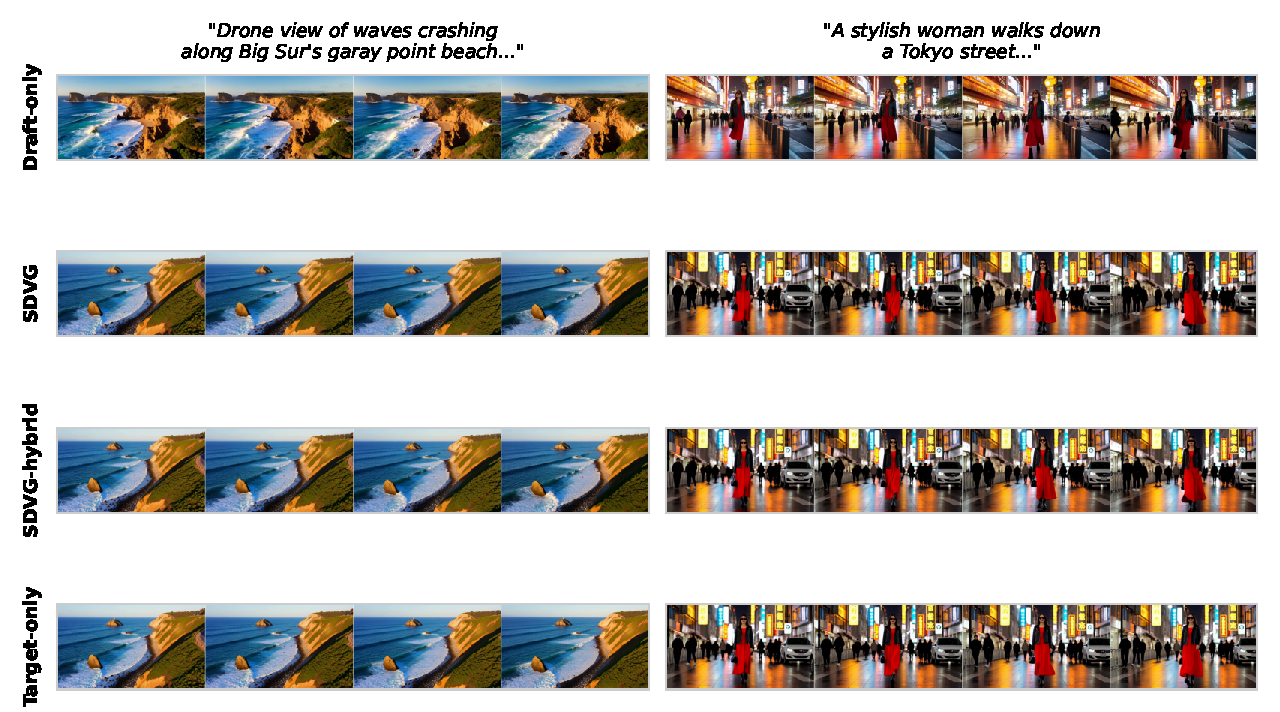
\includegraphics[width=\linewidth]{figures/teaser}
    \caption{%
      \textbf{Qualitative comparison on MovieGenVideoBench.}
      Each cell shows four uniformly sampled frames. Rows compare
      draft-only, \texttt{SDVG}, \texttt{SDVG}-hybrid, and target-only;
      columns show Big Sur and Tokyo street prompts.
      \texttt{SDVG} ($\tau{=}{-}0.7$) closely matches target quality at
      \textbf{1.59$\times$} speedup; \texttt{SDVG}-hybrid
      ($k{=}3$, $\tau{=}{-}1.0$, cascade) reaches \textbf{1.96$\times$}.
    }
    \label{fig:teaser}
  \end{figure}%
}

%%%%%%%%%%%%%%%%%%%%%%%%%%%%%%%%%%%%%%%%%%%%%%%%%%%%%%%%%%%%%%%%%%%%%%%%%%%%
% \section{Introduction}

% Autoregressive video generation has recently emerged as a compelling
% paradigm for efficient, streaming video synthesis.
% Unlike conventional video diffusion models that generate all frames
% jointly \citep{videoworldsimulators2024,polyak2024movie}, autoregressive approaches
% produce video block by block, conditioning each new block on previously
% generated content through a shared key-value (KV) cache, which mirrors the
% autoregressive paradigm of large language models (LLMs).
% This design eliminates exposure bias and enables streaming generation:
% frames can be displayed as they are produced, rather than waiting for the
% full sequence to complete.
% Self-Forcing \citep{huang2025selfforcingbridgingtraintest} exemplifies this approach, training
% a causal video diffusion transformer with self-generated conditioning that
% achieves real-time video output on a single GPU.

% Despite this structural efficiency advantage, state-of-the-art
% autoregressive video models are built on 10B+ parameter transformers, which is still computationally demanding.
% For example, frontier open-source 14B autoregressive video generation models (\citet{krea_realtime_14b})
% require high-end GPUs (e.g. NVIDIA B200) to achieve real-time throughput.
% Meanwhile, compact 1B-scale video models, such as
%  \citet{wan2025wanopenadvancedlargescale}, run at less than one-quarter of the
% computational cost but produce lower but still reasonable quality.
% Thus, the central question is:

% \begin{center}
% \emph{Can we capture the speed of small
% models while retaining the quality of large ones?}
% \end{center}

% Speculative decoding in large language models (LLMs) \citep{leviathan2023fastinferencetransformersspeculative,chen2023acceleratinglargelanguagemodel} offers a compelling paradigm: a compact draft model proposes candidate tokens, while a large target model verifies them only when necessary. The block-by-block architecture of autoregressive video generation aligns naturally with this strategy. Because each generated block serves as a self-contained spatiotemporal unit before being committed to the key-value (KV) cache, it provides a natural boundary for per-block verification and routing.

% However, enabling seamless cooperation between large and small models in video synthesis remains non-trivial. Existing collaborative paradigms fall short in autoregressive contexts: step-level stitching methods (e.g., T-Stitch \citep{pan2024tstitchacceleratingsamplingpretrained}, SRDiffusion \citep{cheng2025srdiffusionacceleratevideodiffusion}, and HybridStitch \citep{sun2026hybridstitch}) split the denoising trajectory across timesteps rather than spatial/temporal blocks, ignoring the causal autoregressive structure. On the other hand, system-level routing schemes like MoDM \citep{xia2025modmefficientservingimage} rely on global cache hits and fail to offer per-block quality guarantees. Consequently, these approaches yield suboptimal performance for autoregressive video generation.

% Crucially, a fundamental domain gap prevents the direct application of LLM speculative decoding to video: while classical speculative decoding verifies drafts via exact token probability distributions \citep{leviathan2023fastinferencetransformersspeculative}, video blocks are continuous, high-dimensional spatiotemporal tensors lacking discrete logits. Thus, standard token-level acceptance criteria are strictly inapplicable, leaving \emph{speculative decoding for autoregressive video} an open challenge.

% In this work, we propose \textbf{Speculative Decoding for Autoregressive Video Generation} (\textbf{\texttt{SDVG}}), a training-free, plug-and-play framework that requires no architectural modifications to either the draft or target models. Our primary contributions are summarized as follows:
% \begin{itemize}
%   \item \textbf{Pioneering Speculative Decoding for Autoregressive Video}: To the best of our knowledge, \texttt{SDVG} is the \textbf{first} training-free speculative decoding framework tailored for autoregressive video diffusion. By dynamically routing video blocks via reward-guided quality metrics, \texttt{SDVG} achieves a $1.59\times$ speedup while preserving $98.1\%$ of the target model's visual quality—demonstrating that plain reward routing suffices without complex trajectory engineering.
%   \item \textbf{Video-Specific Routing Design}: We identify three critical design choices essential for effective continuous-domain verification: (1) a calibration-free quality threshold acting as a robust speed--quality control knob, (2) mandatory target-based first-block generation to anchor scene composition, and (3) a worst-frame quality scoring strategy that exposes transient single-frame artifacts obscured by block-level spatial averaging.
%   \item \textbf{Pushing Acceleration Limits via \texttt{SDVG}-Hybrid}: We further extend our framework into \texttt{SDVG}-hybrid by synergizing block-level speculation with step-level denoising trajectory stitching. By delegating initial denoising steps of rejected blocks to the draft model and incorporating an on-demand evaluation cascade, \texttt{SDVG}-hybrid achieves up to a $1.96\times$ speedup with $96.9\%$ quality retention, significantly outperforming aggressive thresholding on \texttt{SDVG} alone.
% \end{itemize}

\section{Introduction}

Autoregressive video generation has recently emerged as a compelling paradigm for efficient, streaming video synthesis. Unlike conventional video diffusion models that generate all frames jointly \citep{videoworldsimulators2024,polyak2024movie}, autoregressive approaches produce video content block by block, conditioning each new block on previously generated context through a shared key-value (KV) cache—mirroring the autoregressive framework of large language models (LLMs). This design naturally enables streaming generation, allowing frames to be displayed progressively as they are synthesized rather than waiting for the entire sequence to complete. Building on this paradigm, recent frameworks such as Self-Forcing \citep{huang2025selfforcingbridgingtraintest} train causal video diffusion transformers with self-generated conditioning to mitigate exposure bias, enabling real-time streaming video output on a single GPU.

Despite these structural advantages, state-of-the-art autoregressive video models heavily rely on massive architectures ($10\text{B}+$ parameters), incurring severe computational overhead. For instance, frontier open-source 14B autoregressive models \citep{krea_realtime_14b} require enterprise-grade hardware (e.g., NVIDIA B200 GPUs) to attain real-time throughput. Conversely, compact 1B-scale models \citep{wan2025wanopenadvancedlargescale} operate at less than a quarter of the computational cost, albeit with a noticeable compromise in visual fidelity. This stark trade-off leads to our central research question:

\begin{center}
\emph{Can we capture the speed of small models while retaining the generation quality of large ones?}
\end{center}

Speculative decoding in large language models (LLMs) \citep{leviathan2023fastinferencetransformersspeculative,chen2023acceleratinglargelanguagemodel} offers a compelling paradigm: a compact draft model proposes candidate tokens, while a large target model verifies them only when necessary. The block-by-block architecture of autoregressive video generation aligns naturally with this strategy. Because each generated block serves as a self-contained spatiotemporal unit before being committed to the key-value (KV) cache, it provides a natural boundary for per-block verification and dynamic model routing.

However, enabling seamless cooperation between large and small models in video synthesis remains non-trivial. Existing collaborative inference paradigms fall short in autoregressive contexts: step-level stitching methods (e.g., T-Stitch \citep{pan2024tstitchacceleratingsamplingpretrained}, SRDiffusion \citep{cheng2025srdiffusionacceleratevideodiffusion}, and HybridStitch \citep{sun2026hybridstitch}) split the denoising trajectory across timesteps rather than spatial/temporal blocks, ignoring the causal autoregressive structure. On the other hand, system-level routing schemes like MoDM \citep{xia2025modmefficientservingimage} rely on global cache hits and fail to offer per-block quality guarantees. Consequently, these approaches yield suboptimal performance for autoregressive video generation.

Crucially, a fundamental domain gap prevents the direct application of LLM speculative decoding to video: while classical speculative decoding verifies drafts via exact token probability distributions \citep{leviathan2023fastinferencetransformersspeculative}, video blocks are continuous, high-dimensional spatiotemporal tensors lacking discrete logits. Thus, standard token-level acceptance criteria are strictly inapplicable, leaving \emph{speculative decoding for autoregressive video} an open challenge.

In this work, we propose \textbf{Speculative Decoding for Autoregressive Video Generation} (\textbf{\texttt{SDVG}}), a training-free, plug-and-play framework that requires no architectural modifications to either the draft or target models. Our primary contributions are summarized as follows:
\begin{compactitem}[\textbullet]
  \item \textbf{Pioneering Speculative Decoding for Autoregressive Video}: To the best of our knowledge, \texttt{SDVG} is the \textbf{first} training-free speculative decoding framework tailored for autoregressive video diffusion. By dynamically routing video blocks via reward-guided quality metrics, \texttt{SDVG} achieves a $1.59\times$ speedup while preserving $98.1\%$ of the target model's visual quality—demonstrating that plain reward routing suffices without complex trajectory engineering.
  \item \textbf{Video-Specific Routing Design}: We identify three critical design choices essential for effective continuous-domain verification: (1) a calibration-free quality threshold acting as a robust speed--quality control knob, (2) mandatory target-based first-block generation to anchor scene composition, and (3) a worst-frame quality scoring strategy that exposes transient single-frame artifacts obscured by block-level spatial averaging.
  \item \textbf{Pushing Acceleration Limits via \texttt{SDVG}-Hybrid}: We further extend our framework into \texttt{SDVG}-hybrid by synergizing block-level speculation with step-level denoising trajectory stitching. By delegating initial denoising steps of rejected blocks to the draft model and incorporating an on-demand evaluation cascade, \texttt{SDVG}-hybrid achieves up to a $1.96\times$ speedup with $96.9\%$ quality retention, significantly outperforming aggressive thresholding on \texttt{SDVG} alone.
\end{compactitem}

%%%%%%%%%%%%%%%%%%%%%%%%%%%%%%%%%%%%%%%%%%%%%%%%%%%%%%%%%%%%%%%%%%%%%%%%%%%%
\section{Background and Related Work}

\paragraph{Video Generation and Acceleration.}
Diffusion-based video models have evolved from early pixel-space formulations \citep{ho2022videodiffusionmodels} to large latent transformer architectures \citep{videoworldsimulators2024,polyak2024movie}. Inference acceleration in this domain has primarily relied on step distillation \citep{yin2024onestepdiffusiondistributionmatching,zhang2025turbodiffusion,wang2024phased} and GPU kernel optimization \citep{zhang2025sageattention3,zhangspargeattention}. These efficiency-focused techniques operate orthogonally to model architecture routing and can be seamlessly combined with \texttt{SDVG}.

\paragraph{Autoregressive Video Generation.}
Autoregressive video models synthesize future video blocks causally based on previously generated context. Traditional autoregressive training relies on ground-truth historical frames (teacher forcing), creating a fundamental train-test discrepancy that induces severe exposure bias during inference. Recent frameworks, such as Self-Forcing \citep{huang2025selfforcingbridgingtraintest}, mitigate this issue by training causal video diffusion transformers with self-generated conditioning, enabling stable real-time streaming video generation.

\paragraph{Collaborative Multi-Model Inference.}
Collaborative inference leverages models of varying computational capacities to reduce synthesis overhead. For instance, T-Stitch \citep{pan2024tstitchacceleratingsamplingpretrained}, SRDiffusion \citep{cheng2025srdiffusionacceleratevideodiffusion}, and HybridStitch \citep{sun2026hybridstitch} split the denoising trajectory between compact and large models at pre-defined noise levels. System-level approaches like MoDM \citep{xia2025modmefficientservingimage} route whole requests based on global cache hits, reducing average latency. However, these methods rely on content-agnostic timestep partitioning or static caching rules, making them ill-suited for dynamic, block-wise autoregressive video generation.

\paragraph{Speculative Decoding.}
Speculative decoding \citep{leviathan2023fastinferencetransformersspeculative,chen2023acceleratinglargelanguagemodel} pairs a compact draft model with a large target model, where the drafter proposes token sequences that are verified in parallel by the target to strictly preserve the target distribution. Recent work like RSD \citep{liao2025rewardguidedspeculativedecodingefficient} extends speculative verification to reasoning steps via a Process Reward Model (PRM). Inspired by this paradigm, \texttt{SDVG} brings speculative verification to autoregressive video. Because continuous spatiotemporal video tensors lack discrete logit distributions, exact rejection sampling is mathematically inapplicable; we bridge this gap by replacing discrete verification with an image quality model acting as a proxy reward for block-level routing.
%%%%%%%%%%%%%%%%%%%%%%%%%%%%%%%%%%%%%%%%%%%%%%%%%%%%%%%%%%%%%%%%%%%%%%%%%%%%
\begin{figure}[!t]
  \centering
  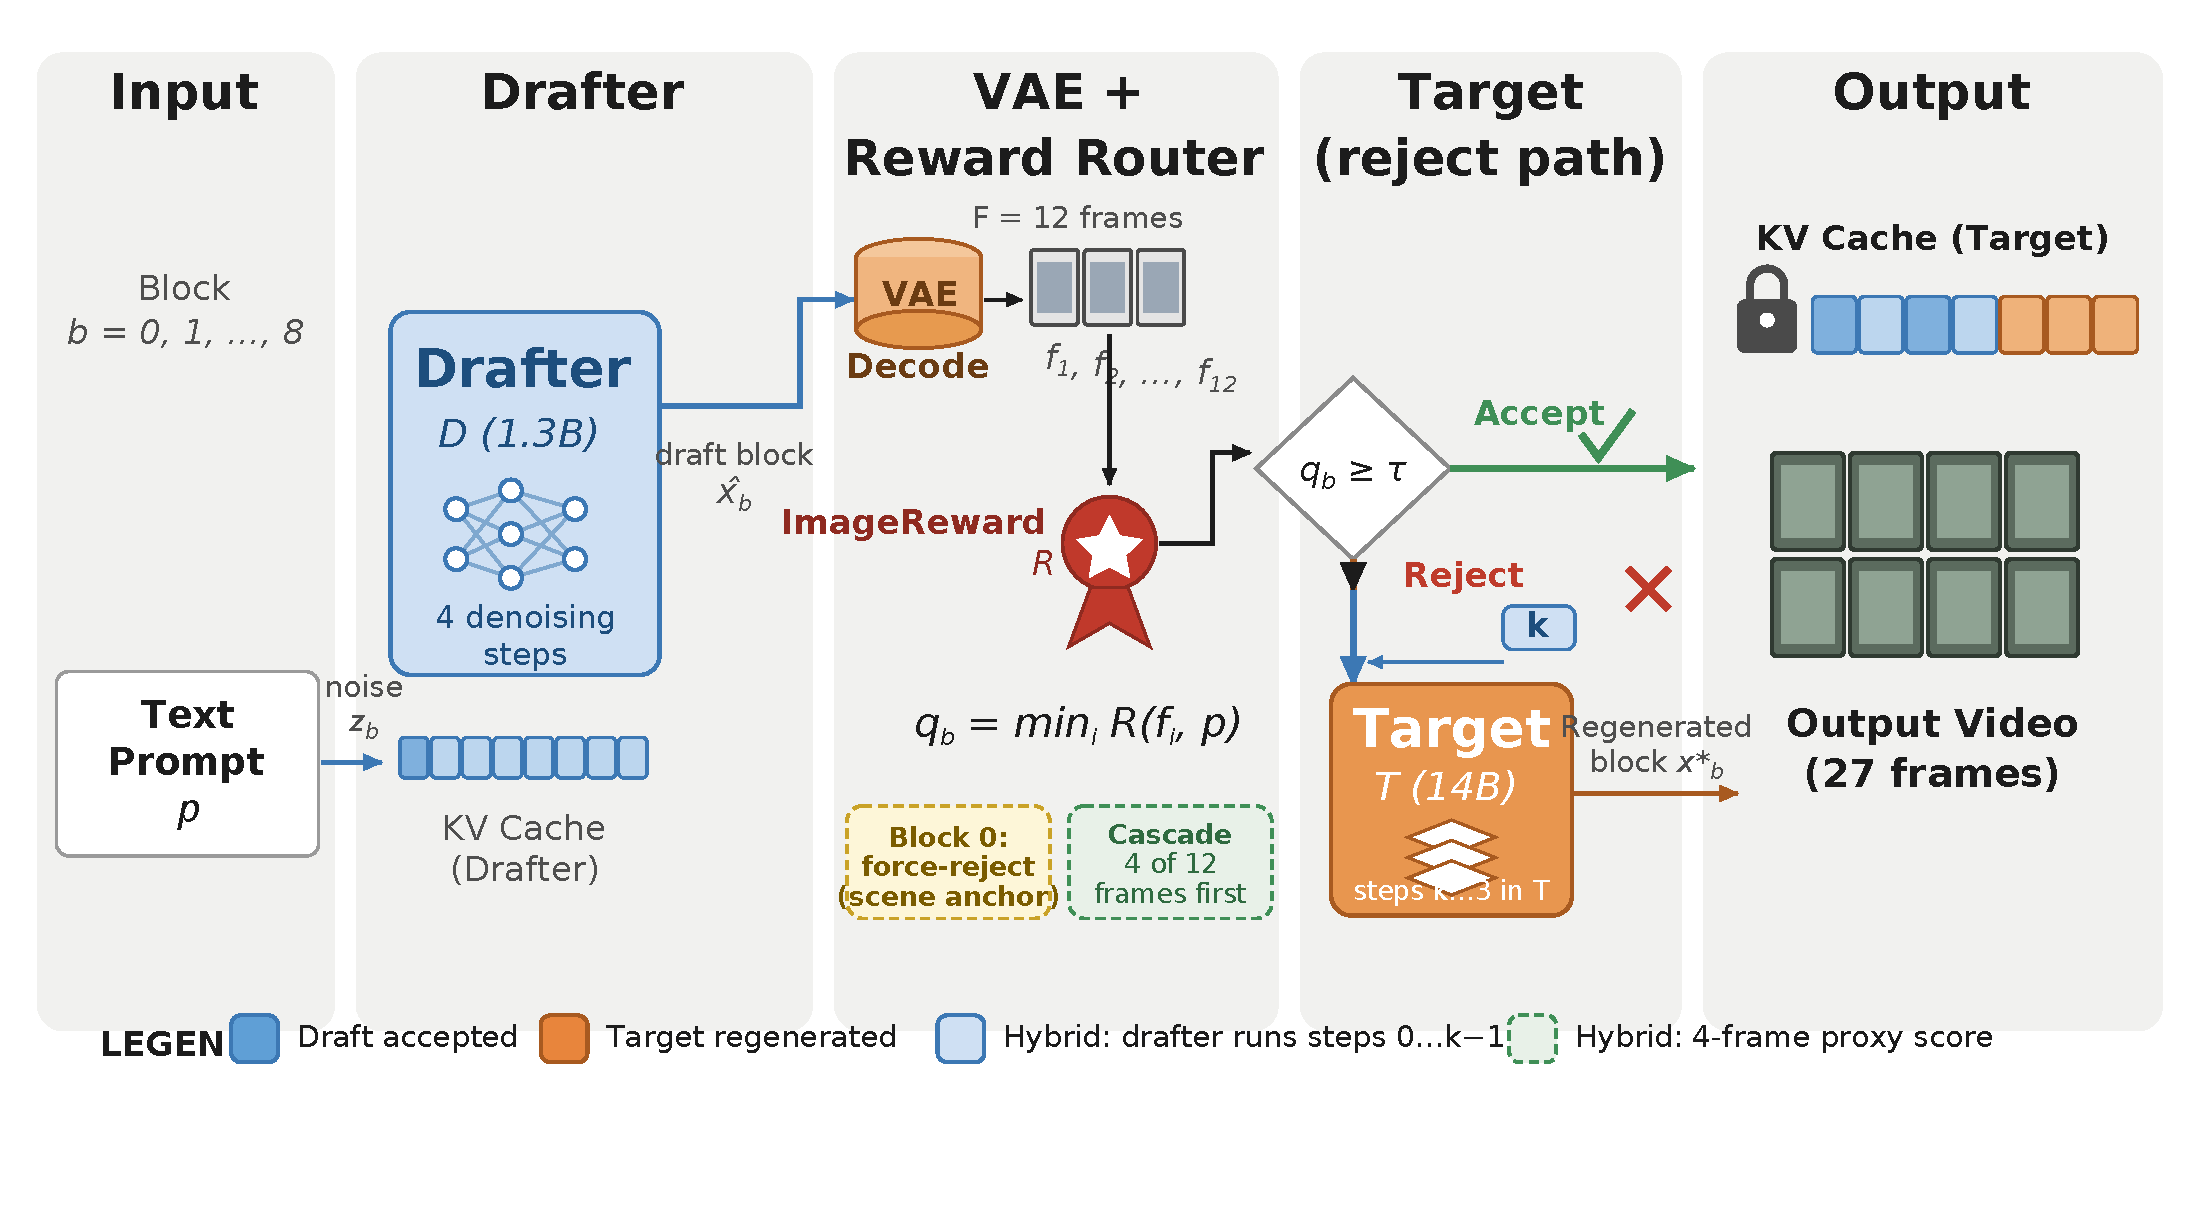
\includegraphics[width=\linewidth]{figures/pipeline}
  \caption{%
    \textbf{Inference pipeline.}
    For each video block, the 1.3B drafter generates a candidate in 4
    denoising steps.
    The draft is VAE-decoded and scored by ImageReward with min-frame
    aggregation ($q_b = \min_i \mathcal{R}(f_i, p)$).
    If $q_b \geq \tau$, the draft is accepted (blue) and committed to the
    target KV cache; otherwise the 14B target regenerates the block
    (orange).
    Block~0 is always force-rejected to anchor scene composition.
    \texttt{SDVG}-hybrid modifies two points of this flow (panels b and c):
    the router scores only 4 of the 12 decoded frames and
    runs the full pass solely when the proxy lands in the grey band, and
    on rejected blocks the target resumes from step~$k$ of the schedule
    rather than from the initial noise, the earlier steps being taken
    from the drafter's trajectory. Block~0 is excluded from stitching.
    % \haocheng{This figure looks too AI-generated. Needs tuning}
  }
  \label{fig:pipeline}
\end{figure}

% \section{Method}
% \label{sec:method}

% This section describes how \texttt{SDVG} brings speculative decoding to
% autoregressive video diffusion. We first present the block-level method
% itself, the inference flow, the worst-frame quality score, and the forced
% regeneration of the first block, and then extend it with
% \texttt{SDVG}-hybrid, which stitches the drafter into the denoising
% trajectory of rejected blocks and resolves most routing decisions from a
% four-frame proxy (Section~\ref{sec:hybrid}).

% \subsection{\texttt{SDVG}: Block-Level Speculation}

% Given text prompt $p$, drafter $\Drafter$ and target $\Target$,
% we seek a routing policy $\pi: \mathbb{R} \to \{0,1\}$ that maps a
% per-block quality score $\score_b \in \mathbb{R}$ to accept (1) or
% reject (0), optimizing the trade-off between video quality and inference
% speed.

% \textbf{Inference flow.}
% For each block $b$, $\Drafter$ runs $S$ denoising steps to produce a
% candidate $\hat{\mathbf{x}}_b$, which is decoded by the VAE and scored by the \emph{router}.
% The router is what stands in for token verification in speculative
% decoding: a lightweight image reward model that judges the block from its
% decoded frames, scoring the whole block as $\score_b$.
% If $\score_b \geq \threshold$, the draft is \emph{accepted}:
% $\hat{\mathbf{x}}_b$ is committed to the target's KV cache
% $\mathbf{K}^{\Target}$ and the decoded frames are emitted directly.
% If \emph{rejected}, $\Target$ regenerates the block and updates
% $\mathbf{K}^{\Target}$.
% The threshold $\threshold$ is a fixed scalar calibrated
% offline.

% \textbf{Worst-frame aggregation.}
% A block is accepted or rejected as a whole, so its score has to describe
% the whole block rather than its average frame: a single frame with a
% broken hand or a smeared face is what a viewer notices, and averaging it
% against all other clean frames would potentially hide it.
% We therefore take the \emph{minimum} per-frame reward over the $F$ decoded
% frames:
% \begin{equation}
%   \score_b = \min_{i=1}^{F}
%   \ImageReward\!\left(\mathbf{f}^{(b)}_i,\, p\right).
%   \label{eq:minscore}
% \end{equation}
% Here $\ImageReward(\mathbf{f}, p)$ denotes the reward of a single decoded
% frame $\mathbf{f}$ given prompt $p$.

% \textbf{Force-reject the first block.}
% At the start of the generation process, block 0 lacks any KV context from prior blocks and establishes the scene
% composition, foreground subjects, and visual style that all subsequent
% blocks inherit through the shared cache.
% Accepting a draft at this position risks propagating irreversible layout
% errors throughout the video. Therefore, block $b=0$ is always routed to $\Target$, regardless of its draft score.









\section{Method}
\label{sec:method}

This section introduces \texttt{SDVG}, a training-free speculative decoding framework tailored for autoregressive video diffusion. We first present the core block-level speculation mechanism (Section~\ref{sec:block_speculation}), detailing its inference workflow, worst-frame quality aggregation, and anchor-block strategy. We then extend this foundation to \texttt{SDVG}-hybrid (Section~\ref{sec:hybrid}), which integrates step-level trajectory stitching with proxy-based routing on rejected blocks to push the limits of computational acceleration.

\subsection{\texttt{SDVG}: Block-Level Speculation}
\label{sec:block_speculation}

Given a text prompt $p$, a compact draft model $\mathcal{D}$, and a large target model $\mathcal{T}$, our goal is to define a routing policy $\pi: \mathbb{R} \to \{0, 1\}$ that maps a per-block quality score $\score_b \in \mathbb{R}$ to a binary decision—accept ($1$) or reject ($0$)—thereby optimizing the throughput--quality trade-off during streaming inference.

\paragraph{Inference Workflow.}
For each autoregressive block $b$, the draft model $\mathcal{D}$ executes $S$ denoising steps to propose a candidate latent block $\hat{\mathbf{x}}_b$. This candidate is subsequently mapped to the pixel domain via a VAE decoder and evaluated by a lightweight router. Serving as the continuous-domain surrogate for token verification in classical speculative decoding, the router evaluates the decoded frames and outputs a scalar quality score $\score_b$. If $\score_b \geq \threshold$, the candidate is \emph{accepted}: $\hat{\mathbf{x}}_b$ is committed to the target model's key-value (KV) cache $\mathbf{K}^{\mathcal{T}}$, and the decoded frames are immediately streamed to output. Conversely, if $\score_b < \threshold$, the draft is \emph{rejected}; the target model $\mathcal{T}$ regenerates the block from scratch, updates $\mathbf{K}^{\mathcal{T}}$, and emits its verified frames. The decision threshold $\threshold$ is a fixed scalar calibrated offline to balance inference speed and visual fidelity.

\paragraph{Worst-Frame Quality Aggregation.}
Because speculative verification is executed per block, the aggregate score $\score_b$ must reflect the visual integrity of the entire temporal segment. Standard spatial or temporal mean-pooling across frames can easily conceal transient perceptual artifacts—such as localized structural distortions or single-frame motion blurs—that remain highly perceptible to human viewers. To prevent artifact propagation, we adopt a conservative \emph{worst-frame} scoring mechanism that takes the minimum reward across all $F$ decoded frames within block $b$:
\begin{equation}
  \score_b = \min_{i=1 \dots F} \mathcal{R}\!\left(\mathbf{f}^{(b)}_i,\, p\right),
  \label{eq:minscore}
\end{equation}
where $\mathcal{R}(\mathbf{f}, p)$ denotes the frame-level quality score computed by a lightweight image reward model (e.g., ImageReward) given prompt $p$.

\paragraph{Mandatory Target Generation for Anchor Block ($b=0$).}
At the onset of generation, the initial block $b=0$ operates without prior context and serves as the global visual anchor—establishing scene composition, spatial layout, and stylistic attributes inherited by all subsequent blocks via the shared KV cache $\mathbf{K}^{\mathcal{T}}$. Accepting an imperfect draft at $b=0$ risks compounding structural degradation throughout the entire video sequence. To anchor high-quality synthesis, we enforce a strict policy: block $b=0$ is always generated by the target model $\mathcal{T}$, bypassing draft evaluation entirely.









% \subsection{\texttt{SDVG}-hybrid: Step-Level Stitching with On-Demand Routing}
% \label{sec:hybrid}

% \texttt{SDVG}'s block-level routing decides \emph{which model} generates a
% block, but it leaves rejected blocks entirely to $\Target$.
% \texttt{SDVG}-hybrid decouples the block axis from the time-step axis:
% rejection hands the target only the denoising steps it is actually needed
% for, not the whole block.
% Since a rejected block no longer discards the drafter's work, the router
% can be both finer-grained and more aggressive about invoking the target.

% \textbf{Step-level stitching.}
% Under \texttt{SDVG}, rejection replays all $S$ target steps from the
% initial noise, discarding the partially denoised state that the scoring
% pass already computed.
% Dropping the replay, we hand the first $k$ steps of every rejected block
% to $\Drafter$ and let $\Target$ finish the trajectory \cite{pan2024tstitchacceleratingsamplingpretrained}:
% \begin{equation}
%   \hat{\mathbf{x}}^{(k)}_b
%   = \Drafter^{\,k}\!\left(\mathbf{z}_b\right),
%   \qquad
%   \mathbf{x}^*_b = \Target^{\,S-k}\!\left(\hat{\mathbf{x}}^{(k)}_b\right),
%   \label{eq:stitch}
% \end{equation}
% where $\Drafter^{\,k}$ denotes $k$ denoising steps of the drafter,
% $\Target^{\,S-k}$ the remaining target steps, and $\mathbf{z}_b$ the
% shared initial noise.
% The stitched steps add no computation. The draft forward passes were
% already paid for during scoring, and the target keeps its final
% low-timestep steps, where its refinement matters most.
% Since block 0 serves as the anchor that fixes the scene every later block
% attends to, it stays entirely target-generated.
% Only later rejected blocks are stitched when rejection decides that the target's
% output is needed.

% \textbf{On-demand cascade routing.}
% In practice, and we find that this routing cost is not negligible, for each single frame needs to be converted by the VAE and scored by the router.
% To further reduce the cost, we propose a hierarchical scoring mechanism.
% A subset of $F_{\mathrm{c}}{=}4$ evenly
% spaced frames serve as a proxy, and is used to generate a preliminary minimum score $\hat{\score}_b$. \texttt{SDVG}-hybrid only falls back to
% the full $F$-frame score when that proxy is inconclusive:
% \begin{equation}
%   \hat{\score}_b \geq \threshold + \delta
%   \;\Rightarrow\; \text{accept},
%   \qquad
%   \hat{\score}_b \leq \threshold - \delta
%   \;\Rightarrow\; \text{reject},
%   \label{eq:cascade}
% \end{equation}
% with the full score computed only when
% $\hat{\score}_b \in (\threshold-\delta, \threshold+\delta)$ for some
% margin $\delta$.
% In our runs only $9.1\%$ of blocks land in that band at
% $\threshold{=}{-}1.0$, so most decisions cost $F_{\mathrm{c}}/F$ of a
% scoring pass; a scorer with a smaller fixed per-call overhead would widen
% this saving further.

\subsection{\texttt{SDVG}-Hybrid: Step-Level Stitching with On-Demand Routing}
\label{sec:hybrid}

While standard \texttt{SDVG} operates purely at the block level—relegating rejected blocks entirely to the target model $\mathcal{T}$—\texttt{SDVG}-hybrid decouples the spatial-temporal block axis from the denoising timestep axis. Upon rejection, rather than discarding candidate latents and re-evaluating from scratch, \texttt{SDVG}-hybrid delegates only the necessary terminal denoising steps to $\mathcal{T}$. Reusing intermediate draft compute allows the router to adopt finer-grained control and a more aggressive acceptance policy.

\paragraph{Step-Level Trajectory Stitching.}
In standard \texttt{SDVG}, a rejected block triggers a full target re-sampling across all $S$ denoising steps, discarding the intermediate latents computed during candidate generation. To eliminate this compute redundancy, \texttt{SDVG}-hybrid retains the initial $k$ denoising steps executed by $\mathcal{D}$ during evaluation, invoking $\mathcal{T}$ only for the remaining $S-k$ steps \citep{pan2024tstitchacceleratingsamplingpretrained}:
\begin{equation}
  \hat{\mathbf{x}}^{(k)}_b = \mathcal{D}^k(\mathbf{z}_b), \qquad \mathbf{x}^*_b = \mathcal{T}^{S-k}\left(\hat{\mathbf{x}}^{(k)}_b\right),
  \label{eq:stitch}
\end{equation}
where $\mathbf{z}_b$ denotes initial Gaussian noise, $\mathcal{D}^k$ represents $k$ denoising steps by the draft model, and $\mathcal{T}^{S-k}$ represents the remaining $S-k$ refinement steps executed by the target model. Because $\hat{\mathbf{x}}^{(k)}_b$ is already obtained during the candidate scoring pass, this step-level stitching adds zero computational overhead while leveraging $\mathcal{T}$ where its capacity matters most (i.e., fine-grained detail generation at low noise levels). As with standard \texttt{SDVG}, the initial anchor block ($b=0$) remains fully generated by $\mathcal{T}$ to preserve global visual coherence.

\paragraph{On-Demand Cascade Routing.}
In practice, decoding every candidate frame via VAE and scoring it through the reward model introduces non-negligible verification overhead. To minimize this bottleneck, we introduce a hierarchical, on-demand scoring mechanism. We first extract a sparse subset of $F_{\mathrm{c}} = 4$ temporally uniform proxy frames to compute a preliminary score $\hat{\score}_b$. The router then conditionally determines whether to fall back to the full $F$-frame evaluation based on a confidence margin $\delta$:
\begin{equation}
  \text{Decision} = 
  \begin{cases} 
  \text{Accept}, & \text{if } \hat{\score}_b \ge \threshold + \delta, \\ 
  \text{Reject}, & \text{if } \hat{\score}_b \le \threshold - \delta, \\ 
  \text{Evaluate } \score_b \text{ on all } F \text{ frames}, & \text{if } \hat{\score}_b \in (\threshold - \delta, \, \threshold + \delta).
  \end{cases}
  \label{eq:cascade}
\end{equation}
When the proxy evaluation yields a decisive result ($\hat{\score}_b \notin (\threshold - \delta, \threshold + \delta)$), full $F$-frame decoding and scoring are completely bypassed, reducing verification cost to $F_{\mathrm{c}}/F$ of the full scoring pass. Empirically, the vast majority of blocks fall outside this ambiguous interval (e.g., only 9.1\% land within $(\threshold - \delta, \threshold + \delta)$ at $\threshold = -1.0$), resulting in significant operational speedups.


%%%%%%%%%%%%%%%%%%%%%%%%%%%%%%%%%%%%%%%%%%%%%%%%%%%%%%%%%%%%%%%%%%%%%%%%%%%%
% \section{Experiments}
% \label{sec:experiments}

% This section provides empirical results of our proposed method.
% We first introduce the models and settings (Section~\ref{sec:setup}),
% then present the quality--speed trade-off of both \texttt{SDVG} and
% \texttt{SDVG}-hybrid (Section~\ref{sec:main-results}), and close with
% ablations of both methods that isolate which design choices carry the
% gains (Section~\ref{sec:ablation}).

% \subsection{Experimental Setup}
% \label{sec:setup}

% \paragraph{Models.}
% We evaluate \texttt{SDVG} on a pair of autoregressive video diffusion models built
% on the Wan2.1 architecture \citep{wan2025wanopenadvancedlargescale}.
% The \emph{target model} is Krea Realtime Video 14B \citep{krea_realtime_14b},
% distilled from Wan2.1-T2V-14B via Self-Forcing \citep{huang2025selfforcingbridgingtraintest}.
% The \emph{drafter} is the original Wan2.1-T2V-1.3B Self-Forcing model.
% Both models share the same causal attention backbone with KV caching via
% RoPE positional embeddings, and run 4 denoising steps per block using the
% schedule $\mathbf{t} = [1000, 937, 833, 625, 0]$.
% The reward router uses ImageReward \citep{xu2023imagerewardlearningevaluatinghuman}, an
% off-the-shelf text-image reward model, to score decoded draft frames.

% \paragraph{Generation protocol.}
% Each video consists of $B{=}9$ autoregressive blocks. Each block corresponds to 3 latent frames (27 latent frames in total). The causal VAE
% decoder produces $9$ pixel frames for the first video block and $12$ pixel frames per later video block at $832 \times 480$ resolution.
% All runs use a fixed random seed (42) for reproducibility.

% \paragraph{Hardware and implementation.}
% All experiments are conducted on two NVIDIA RTX A6000 GPUs (48\,GB each).
% GPU\,0 hosts the diffusion transformer (both target and drafter);
% GPU\,1 hosts the text encoder (UMT5-XXL), causal VAE, and ImageReward.
% CUDA streams overlap cross-device transfers with compute so that reward
% scoring does not block denoising.

% \paragraph{Evaluation benchmarks and metrics.}
% We draw prompts from MovieGenVideoBench \citep{polyak2024movie}, which
% spans diverse categories including landscapes, animals, human activities,
% and cinematic footage, totaling a 1003-prompt set.
% Video quality is measured by {VisionReward} \citep{xu2026visionrewardfinegrainedmultidimensionalhuman},
% and EvalCrafter \citep{liu2024evalcrafterbenchmarkingevaluatinglarge}.
% Efficiency is measured by {wall-clock time} per video (excluding
% model loading and warmup), and the resulting {speedup} relative to
% target-only generation.

% \paragraph{Baselines.}
% We compare against two boundary baselines:
% \emph{Draft-only}---all blocks generated by the 1.3B drafter
% (maximum speed, lowest quality);
% \emph{Target-only}---all blocks generated by the 14B target
% (minimum speed, highest quality).
% \texttt{SDVG} and \texttt{SDVG}-hybrid operates between these extremes by sweeping the routing threshold,
% the number of stitched denoising steps, and whether
% on-demand cascade scoring is enabled.

\section{Experiments}
\label{sec:experiments}

In this section, we empirically evaluate the performance and efficiency of \texttt{SDVG} and \texttt{SDVG}-hybrid. We first outline the base models, hardware infrastructure, and evaluation protocols (Section~\ref{sec:setup}). We then analyze the Pareto trade-offs between video quality and generation speed against boundary baselines (Section~\ref{sec:main-results}). Finally, we conduct thorough ablation studies to isolate the individual contributions of key architectural components, including worst-frame quality aggregation, anchor block generation, and on-demand cascade routing (Section~\ref{sec:ablation}).

\subsection{Experimental Setup}
\label{sec:setup}

We pair a Krea Realtime Video 14B target \citep{krea_realtime_14b} with a Wan2.1-T2V-1.3B Self-Forcing draft and use ImageReward \citep{xu2023imagerewardlearningevaluatinghuman} for routing. On $1{,}003$ MovieGenVideoBench prompts \citep{polyak2024movie}, each method generates nine video blocks at $832\times480$ using two NVIDIA RTX A6000 GPUs. We report VisionReward, EvalCrafter, latency per video, and speedup over target-only; draft-only and target-only bound the quality--speed range. Appendix~\ref{app:setup} provides the denoising schedule, decoding protocol, hardware configuration, baseline definitions, and reproducibility details.


% \subsection{Main Results}
% \label{sec:main-results}

% Table~\ref{tab:main} reports the two sweeps we compare---\texttt{SDVG} with
% its min-frame threshold varying, and \texttt{SDVG}-hybrid at the matched
% thresholds---against the two boundary baselines, and
% Figure~\ref{fig:pareto} plots the same numbers against speedup.
% The table's lower panel adds EvalCrafter's raw metrics for the same
% settings.
\subsection{Main Results}
\label{sec:main-results}

We systematically evaluate \texttt{SDVG} and \texttt{SDVG}-hybrid across various quality thresholds $\threshold$, benchmarking them against the boundary \emph{Draft-only} ($\mathcal{D}$-only) and \emph{Target-only} ($\mathcal{T}$-only) baselines. Table~\ref{tab:main} summarizes the overall quality--speed trade-offs on MovieGenVideoBench alongside fine-grained EvalCrafter metrics, while Figure~\ref{fig:pareto} illustrates the corresponding Pareto frontiers.


\begin{table}[t]
  \caption{%
    \textbf{Main results on MovieGenVideoBench.}
    \texttt{SDVG} and \texttt{SDVG}-hybrid across the routing threshold.
    VR is VisionReward, higher being better, and Ret.\ is the same
    quantity expressed as a percentage of target-only.
    Every \texttt{SDVG}-hybrid row stitches $k{=}3$ denoising steps of a
    rejected block and resolves most routing decisions from a four-frame
    proxy before falling back on all twelve, leaving block~0 to the
    target, so the rows differ only in the threshold.
    The lower panel reports EvalCrafter's raw metrics for the same
    settings, with the arrows following the direction that benchmark's
    fitted aggregation rewards (for IS, action score and flow score,
    lower is better) and with \emph{warp} denoting the optical-flow
    warping error, \emph{BLEU} the BLIP caption BLEU, and \emph{detect}
    the object detection rate.
  }
  \label{tab:main}
  \centering
  \small
  \begin{tabular*}{0.97\linewidth}{@{\extracolsep{\fill}}llcccccc}
    \toprule
    Method & $\tau$ & VR $\uparrow$ & Ret.\ (\%) & Time (s) & Speedup & Accept \\
    \midrule
    Target-only        & ---    & 0.0788 & 100.0 & 97.0 & 1.00$\times$ & ---    \\
    \midrule
    \texttt{SDVG}      & $-0.7$ & 0.0773 & 98.10 & 60.9 & 1.59$\times$ & 73.1\% \\
    \texttt{SDVG}      & $-1.0$ & 0.0764 & 96.95 & 57.2 & 1.69$\times$ & 78.0\% \\
    \texttt{SDVG}      & $-1.5$ & 0.0757 & 96.07 & 51.6 & 1.88$\times$ & 83.4\% \\
    \texttt{SDVG}      & $-2.0$ & 0.0756 & 95.94 & 47.4 & 2.05$\times$ & 87.5\% \\
    \midrule
    \texttt{SDVG}-hybrid & $-0.7$ & 0.0772 & 97.97 & 51.6 & 1.88$\times$ & 72.8\% \\
    \texttt{SDVG}-hybrid & $-1.0$ & 0.0764 & 96.95 & 49.5 & 1.96$\times$ & 77.5\% \\
    \texttt{SDVG}-hybrid & $-1.5$ & 0.0759 & 96.32 & 48.2 & 2.01$\times$ & 83.2\% \\
    \texttt{SDVG}-hybrid & $-2.0$ & 0.0751 & 95.30 & 46.1 & 2.11$\times$ & 87.4\% \\
    \midrule
    Draft-only         & ---    & 0.0644 & 81.73 & 25.7 & 3.77$\times$ & ---    \\
    \bottomrule
  \end{tabular*}

  \vspace{7pt}
  \small
  \begin{tabular*}{0.97\linewidth}{@{\extracolsep{\fill}}llccccccc}
    \toprule
    Method & $\tau$ & VQA\_T $\uparrow$ & IS $\downarrow$ & warp $\downarrow$
           & action $\downarrow$ & flow $\downarrow$
           & BLEU $\uparrow$ & detect $\uparrow$ \\
    \midrule
    Target-only        & ---    & 93.33 & 18.62 & 0.0066 & 45.18 & 4.99 & 21.66 & 78.09 \\
    \midrule
    \texttt{SDVG}      & $-0.7$ & 93.11 & 18.99 & 0.0085 & 45.38 & 5.16 & 21.92 & 77.85 \\
    \texttt{SDVG}      & $-1.0$ & 93.08 & 19.17 & 0.0088 & 45.29 & 5.18 & 21.89 & 78.44 \\
    \texttt{SDVG}      & $-1.5$ & 92.81 & 19.15 & 0.0090 & 45.28 & 5.31 & 21.74 & 78.54 \\
    \texttt{SDVG}      & $-2.0$ & 93.04 & 19.20 & 0.0092 & 45.45 & 5.35 & 21.73 & 78.70 \\
    \midrule
    \texttt{SDVG}-hybrid & $-0.7$ & 92.94 & 19.13 & 0.0089 & 45.49 & 5.39 & 21.87 & 78.19 \\
    \texttt{SDVG}-hybrid & $-1.0$ & 92.94 & 19.01 & 0.0091 & 45.38 & 5.38 & 21.88 & 77.88 \\
    \texttt{SDVG}-hybrid & $-1.5$ & 93.13 & 19.12 & 0.0092 & 45.47 & 5.37 & 21.86 & 77.90 \\
    \texttt{SDVG}-hybrid & $-2.0$ & 92.98 & 19.08 & 0.0092 & 45.48 & 5.36 & 21.78 & 77.82 \\
    \midrule
    Draft-only         & ---    & 92.75 & 19.52 & 0.0102 & 46.95 & 5.90 & 21.00 & 72.57 \\
    \bottomrule
  \end{tabular*}
\end{table}

% \paragraph{Quality--time tradeoff.}
% Sweeping $\tau$ from $-0.7$ to $-2.0$ traces a smooth Pareto frontier
% between the two baselines (Figure~\ref{fig:pareto}).
% At the conservative end ($\tau{=}{-}0.7$) \texttt{SDVG} keeps ${98.10\%}$ of
% target-only VisionReward (0.0773 vs.\ 0.0788) at a \textbf{1.59$\times$}
% speedup; relaxing the threshold to $-1.0$ buys ${1.69\times}$ for
% ${96.95\%}$; and at the aggressive end ($\tau{=}{-}2.0$) it reaches
% \textbf{2.05$\times$} at ${95.94\%}$, still $+17.4\%$ above draft-only
% (0.0756 vs.\ 0.0644).
% The gains flatten past $\tau{=}{-}1.5$: most quality-critical blocks
% already score above $-1.5$, so further relaxation buys little speed and
% costs quality instead.

% \paragraph{Quality--acceptance rate tradeoff.}
% Seen against the acceptance rate, the same frontier is nearly flat at the
% conservative end: moving from 73.1\% ($\tau{=}{-}0.7$) to 78.0\%
% ($\tau{=}{-}1.0$) costs $1.2\%$ relative VisionReward
% (0.0773 $\to$ 0.0764).
% The drafts admitted in that range are borderline cases whose quality is
% close to what the target would have produced, which is exactly what a
% reward-guided router should let through.
% Past 78\% the slope steepens---83.4\% acceptance costs 0.0757 and 87.5\%
% costs 0.0756---as low-scoring drafts start to slip in.
% The knee at $\tau \in [-1.0, -0.7]$ (73--78\% acceptance) is therefore the
% operating regime with the best quality--efficiency balance.

% \paragraph{\texttt{SDVG}-hybrid extends the frontier.}
% Adding step-level stitching ($k{=}3$, block~0 left to the target) and
% on-demand cascade scoring at $\tau{=}{-}1.0$ gives 0.0764 VisionReward at
% 49.5\,s, a \textbf{1.96$\times$} speedup at ${96.9\%}$ of target quality.
% That point beats \texttt{SDVG} $\tau{=}{-}1.5$ on both axes---faster and
% higher-quality---and it matches \texttt{SDVG} $\tau{=}{-}1.0$ in quality
% while running ${1.96\times}$ instead of ${1.69\times}$: stitching recovers
% the target's trajectory instead of replaying it, and the cascade removes
% most of the scoring cost.
% The advantage narrows as both sweeps approach $2\times$: the aggressive
% \texttt{SDVG} thresholds reach the same region, and the hybrid's
% $\tau{=}{-}2.0$ point buys its last $0.06\times$ by slipping to $95.3\%$
% retention.
% Section~\ref{sec:ablation} separates the two contributions.

\paragraph{Quality--Speed Trade-Off.}
Varying the minimum-frame threshold $\threshold$ from $-0.7$ to $-2.0$ traces a smooth Pareto frontier between the two baseline models (Figure~\ref{fig:pareto}). Under conservative thresholding ($\threshold = -0.7$), \texttt{SDVG} retains $98.10\%$ of target-only VisionReward ($0.0773$ vs. $0.0788$) while delivering a $\mathbf{1.59\times}$ speedup. Relaxing the threshold to $\threshold = -1.0$ accelerates inference to $\mathbf{1.69\times}$ with $96.95\%$ quality retention. Even under aggressive thresholding ($\threshold = -2.0$), \texttt{SDVG} achieves a $\mathbf{2.05\times}$ speedup while preserving $95.94\%$ of target quality—outperforming the \emph{Draft-only} baseline by $+17.4\%$ in VisionReward ($0.0756$ vs. $0.0644$). Latency gains exhibit diminishing returns beyond $\threshold = -1.5$: because most quality-critical blocks naturally clear this threshold, further relaxation yields marginal speed improvements at the expense of visual fidelity.

\paragraph{Quality--Acceptance Rate Relationship.}
Analyzing visual quality relative to block acceptance rates reveals a highly favorable regime at conservative thresholds. Increasing the acceptance rate from $73.1\%$ ($\threshold = -0.7$) to $78.0\%$ ($\threshold = -1.0$) results in only a minimal $1.2\%$ relative decline in VisionReward ($0.0773 \to 0.0764$). This confirms that the router effectively admits borderline draft candidates whose visual quality closely matches target-generated outputs. Beyond $78\%$ acceptance, quality degradation accelerates—dropping to $0.0757$ at $83.4\%$ acceptance and $0.0756$ at $87.5\%$—as sub-optimal draft blocks are increasingly admitted. Consequently, the threshold interval $\threshold \in [-1.0, -0.7]$ (corresponding to $73\%\text{--}78\%$ block acceptance) represents the optimal operating regime for balancing quality and efficiency.

\paragraph{Pareto Extension via \texttt{SDVG}-Hybrid.}
Integrating step-level trajectory stitching ($k=3$) and on-demand cascade routing into \texttt{SDVG}-hybrid significantly expands the Pareto frontier. At $\threshold = -1.0$, \texttt{SDVG}-hybrid achieves a $\mathbf{1.96\times}$ speedup ($49.5\text{~s}$ per video) while preserving $96.9\%$ of target quality ($0.0764$ VisionReward). This operating point strictly dominates standard \texttt{SDVG} at $\threshold = -1.5$ across both speed and quality dimensions. Furthermore, compared to standard \texttt{SDVG} at the same threshold ($\threshold = -1.0$), \texttt{SDVG}-hybrid boosts acceleration from $1.69\times$ to $1.96\times$ with zero degradation in visual quality. This improvement stems from two factors: trajectory stitching reuses intermediate draft latents instead of replaying full target denoising, while cascade routing eliminates redundant VAE decoding and reward evaluation overheads. The relative advantage of the hybrid model narrows as generation approaches $2.0\times$ acceleration, where permissive thresholds allow draft quality limits to dominate runtime savings. We disentangle these individual mechanisms in Section~\ref{sec:ablation}.


\begin{figure}[t]
  \centering
  \begin{minipage}[c]{0.34\linewidth}
    \captionsetup{justification=raggedright,singlelinecheck=false}
    \caption{%
      \textbf{Quality--speed Pareto curve.}
      VisionReward against speedup over target-only for the threshold sweeps
      of \texttt{SDVG} and \texttt{SDVG}-hybrid; the dashed line is
      target-only.
      The \texttt{SDVG}-hybrid curve sits above the \texttt{SDVG} curve
      through $2.0\times$, with the gap widest at the conservative end:
      hybrid $\tau{=}{-}0.7$ matches \texttt{SDVG} $\tau{=}{-}0.7$ quality
      9.3\,s sooner.
    }
    \label{fig:pareto}
  \end{minipage}\hspace{0.04\linewidth}
  \begin{minipage}[c]{0.50\linewidth}
    \centering
    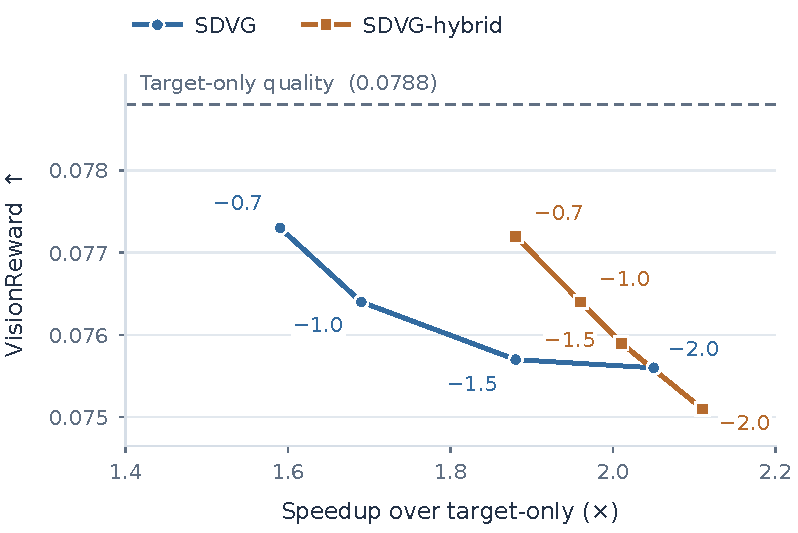
\includegraphics[width=\linewidth]{figures/quality_speed_tradeoff}
  \end{minipage}
\end{figure}

% \subsection{Ablation Studies}
% \label{sec:ablation}

% We ablate both methods. Table~\ref{tab:ablation} varies the two design
% choices behind \texttt{SDVG}---how a block is scored and what signal the
% router acts on---and Table~\ref{tab:hybrid} takes \texttt{SDVG}-hybrid
% apart one factor at a time. Every run keeps the force-reject-block-0
% policy, so the comparisons stay controlled.

% \paragraph{Reward-guided vs.\ random routing.}
% To check that the ImageReward signal is load-bearing, we replace the
% reward router with random accept/reject decisions at a matched acceptance
% rate. VisionReward falls to 0.0706, below every other row in the table and
% $0.0067$ under the reward-guided \texttt{SDVG} at $\tau{=}{-}0.7$: without
% a quality signal the router admits artifact-heavy blocks and turns away
% clean ones at the same rate, which cancels the benefit of selective
% regeneration.
% Two rows bracket what the router is worth. Keeping the force-reject policy
% and nothing else---every other draft accepted, no scoring---recovers 0.0757
% at ${2.21\times}$ and is the fastest setting that keeps block~0
% target-generated; the same random router on top of that policy reaches
% 0.0771, so block~0 alone accounts for most of the gap between random
% routing and the full method.

% \paragraph{Min-frame vs.\ average-frame scoring.}
% Our default \texttt{SDVG} scores a block by its worst frame
% (Eq.~\ref{eq:minscore}), so it flags the block as soon as one frame is
% degraded. Average-frame variants never close the gap at comparable
% acceptance rates---0.0755 at 78.4\% against 0.0773 at 73.1\% for min-frame
% $\tau{=}{-}0.7$---because a single corrupted frame among the $F$ the block
% decodes carries visible temporal flickering that the mean absorbs.

\subsection{Ablation Studies}
\label{sec:ablation}

We conduct comprehensive ablation studies to isolate the individual contributions of key components in \texttt{SDVG} and \texttt{SDVG}-hybrid. Table~\ref{tab:ablation} evaluates the foundational design choices of block-level speculation—specifically the choice of routing signal and frame-level score aggregation. Table~\ref{tab:hybrid} systematically deconstructs \texttt{SDVG}-hybrid across stitching depths $k$, anchor-block protection policies, and cascade thresholds. All experimental configurations enforce mandatory target generation for the anchor block ($b=0$) unless explicitly noted otherwise.

\paragraph{Efficacy of Reward-Guided Routing.}
To verify that the ImageReward signal provides meaningful quality guidance, we replace the reward router with random accept/reject decisions matched to an identical acceptance rate ($70.0\%$). As shown in Table~\ref{tab:ablation}, random routing causes VisionReward to drop sharply to $0.0706$—a $0.0067$ decrease compared to reward-guided \texttt{SDVG} at $\threshold = -0.7$. Lacking visual awareness, the random router frequently admits artifact-laden drafts while rejecting high-quality candidates at equal rates, completely negating the benefit of selective regeneration. 

To delineate the utility bounds of our policy, we evaluate a baseline that enforces anchor block protection ($b=0$) while unconditionally accepting all subsequent draft blocks without verification. This naive policy achieves $0.0757$ VisionReward at $2.21\times$ speedup. Applying random routing on top of this policy yields $0.0771$, indicating that while protecting the anchor block provides a crucial structural foundation, dynamic reward-guided routing is indispensable for recovering near-target visual quality.

\paragraph{Worst-Frame vs. Mean-Frame Aggregation.}
Standard \texttt{SDVG} evaluates candidate blocks via worst-frame aggregation (Eq.~\ref{eq:minscore}), flagging a block as soon as a single frame exhibits visual degradation. As reported in Table~\ref{tab:ablation}, mean-pooling variants consistently underperform worst-frame aggregation at comparable acceptance rates ($0.0755$ at $78.4\%$ acceptance for mean-pooling vs. $0.0773$ at $73.1\%$ for worst-frame at $\threshold = -0.7$). This disparity arises because temporal mean-pooling across $F$ frames absorbs localized structural distortions and single-frame motion artifacts, allowing corrupted blocks to pass verification undetected.

% \begin{table}[t]
%   \caption{%
%     \textbf{Ablation study.}
%     1003 MovieGenVideoBench prompts, $832{\times}480$, 9 blocks/video.
%     VR = VisionReward (higher is better).
%     Time = average wall-clock time per video.
%     Accept rate is over all nine blocks, so the always-rejected block~0
%     counts as a rejection.
%     ``---'' indicates not applicable.
%   }
%   \label{tab:ablation}
%   \centering
%   \setlength{\tabcolsep}{13pt}
%   \begin{tabular}{lcccc}
%     \toprule
%     Method & VR $\uparrow$ & Time (s) & Speedup & Accept \\
%     \midrule
%     Target-only                       & 0.0788 & 97.0 & 1.00$\times$ & ---    \\
%     \midrule
%     \textbf{\texttt{SDVG} ($\tau{=}{-}0.7$, ours)} & \textbf{0.0773} & 60.9 & 1.59$\times$ & 73.1\% \\
%     \midrule
%     \multicolumn{5}{l}{\textit{Avg-frame scoring (replacing min-frame)}} \\
%     Avg-frame $\tau{=}{-}0.2$         & 0.0767 & 63.2 & 1.54$\times$ & 70.2\% \\
%     Avg-frame $\tau{=}{-}0.5$         & 0.0759 & 59.0 & 1.64$\times$ & 75.3\% \\
%     Avg-frame $\tau{=}{-}0.7$         & 0.0755 & 56.9 & 1.71$\times$ & 78.4\% \\
%     \midrule
%     \multicolumn{5}{l}{\textit{Routing signal ablation}} \\
%     Force-reject $+$ random routing   & 0.0771 & 58.2 & 1.67$\times$ & 70.3\% \\
%     Force-reject only, no verification & 0.0757 & 43.8 & 2.21$\times$ & 100.0\% \\
%     Random routing                    & 0.0706 & 60.2  & 1.61$\times$ & 70.0\% \\
%     \midrule
%     Draft-only                        & 0.0644 & 25.7 & 3.77$\times$ & ---    \\
%     \bottomrule
%   \end{tabular}
% \end{table}

% \paragraph{What the hybrid buys.}
% Table~\ref{tab:hybrid} lists the full configuration first, then walks
% through one factor at a time---the stitching depth $k$, whether block~0 is
% stitched too, and the routing threshold, with the cascade column giving
% the on/off pair at each threshold---so each mechanism can be read off on
% its own.

% \begin{table}[t]
%   \caption{%
%     \textbf{\texttt{SDVG}-hybrid ablations.}
%     1003 MovieGenVideoBench prompts, $832{\times}480$, 9 blocks/video,
%     min-frame ImageReward.
%     $k$ is the number of denoising steps a rejected block takes from the
%     drafter rather than from the target.
%     Retention is VisionReward relative to target-only (0.0788).
%     The default row is the full configuration and the groups below vary one
%     factor at a time, each naming the settings it changes.
%   }
%   \label{tab:hybrid}
%   \centering
%   \setlength{\tabcolsep}{6pt}
%   \begin{tabular}{lccccc}
%     \toprule
%     Method & Cascade & VR $\uparrow$ & Time (s) & Speedup & Retention \\
%     \midrule
%     Target-only & --- & 0.0788 & 97.0 & 1.00$\times$ & 100.0\% \\
%     \midrule
%     \textbf{\texttt{SDVG}-hybrid ($k{=}3$, $\tau{=}{-}0.7$)}
%       & $\checkmark$ & \textbf{0.0772} & \textbf{51.6} & \textbf{1.88$\times$} & \textbf{98.0\%} \\
%     \textbf{\texttt{SDVG}-hybrid ($k{=}3$, $\tau{=}{-}1.0$, ours)}
%       & $\checkmark$ & \textbf{0.0764} & \textbf{49.5} & \textbf{1.96$\times$} & \textbf{96.9\%} \\
%     \midrule
%     \multicolumn{6}{l}{\textit{Stitching depth ($\tau{=}{-}0.7$, block~0 protected)}} \\
%     $k{=}2$ & $\times$ & 0.0756 & 56.2 & 1.73$\times$ & 95.9\% \\
%     $k{=}3$ & $\times$ & \textbf{0.0766} & 54.3 & 1.79$\times$ & \textbf{97.2\%} \\
%     $k{=}4$ & $\times$ & 0.0752 & 52.5 & 1.85$\times$ & 95.5\% \\
%     \midrule
%     \multicolumn{6}{l}{\textit{Stitching block~0 as well ($\tau{=}{-}0.7$)}} \\
%     $k{=}2$ & $\times$ & 0.0688 & 58.9 & 1.65$\times$ & 87.3\% \\
%     $k{=}3$ & $\times$ & 0.0677 & 51.6 & 1.88$\times$ & 85.9\% \\
%     $k{=}4$ & $\times$ & 0.0646 & 46.7 & 2.08$\times$ & 82.0\% \\
%     \midrule
%     \multicolumn{6}{l}{\textit{Varying the threshold ($k{=}3$, block~0 protected)}} \\
%     $\tau{=}{-}0.7$ & $\times$ & 0.0766 & 54.3 & 1.79$\times$ & 97.2\% \\
%     $\tau{=}{-}0.7$ & $\checkmark$ & 0.0772 & 51.6 & 1.88$\times$ & 98.0\% \\
%     $\tau{=}{-}1.0$ & $\times$ & 0.0763 & 51.7 & 1.88$\times$ & 96.9\% \\
%     $\tau{=}{-}1.0$ & $\checkmark$ & 0.0764 & 49.5 & 1.96$\times$ & 96.9\% \\
%     $\tau{=}{-}1.5$ & $\times$ & 0.0760 & 49.1 & 1.97$\times$ & 96.4\% \\
%     $\tau{=}{-}1.5$ & $\checkmark$ & 0.0759 & 48.2 & 2.01$\times$ & 96.3\% \\
%     $\tau{=}{-}2.0$ & $\times$ & 0.0758 & 49.3 & 1.97$\times$ & 96.2\% \\
%     $\tau{=}{-}2.0$ & $\checkmark$ & 0.0751 & 46.1 & 2.11$\times$ & 95.3\% \\
%     \bottomrule
%   \end{tabular}
% \end{table}

% \paragraph{Step-level stitching.}
% Handing the first $k$ denoising steps of a rejected block back to the
% drafter costs nothing---those forward passes were already paid for during
% scoring---and the partially denoised state it hands over is strictly more
% informative than the initial noise the target would otherwise restart
% from.
% $k{=}3$ is the sweet spot: it matches target quality at 0.0766
% (97.2\% retention) while running ${1.79\times}$ faster.
% Smaller $k$ leaves the target more work to redo, and $k{=}4$ hands over
% the entire four-step schedule, leaving the target nothing to refine---the
% rejected block is then effectively the draft, which is exactly what the
% router rejected, and quality falls to 0.0752.

% \paragraph{Block~0 must stay target-generated.}
% Stitching block~0 as well collapses quality: at $k{=}3$ the same
% configuration drops from 0.0766 to 0.0677 VisionReward, and the damage
% grows with $k$.
% Block~0 has no prior context, so it fixes the scene that every later
% block attends to; letting a truncated drafter trajectory define it
% commits the whole video to a composition the target never refines, and
% the error compounds through the shared cache.

% \paragraph{On-demand cascade.}
% Scoring four of the twelve decoded frames rather than all twelve removes
% most of the routing cost without changing decisions that matter: at
% $\tau{=}{-}1.0$ only $9.1\%$ of blocks fall inside the ambiguity band and
% need the full pass, which saves $2.2$\,s (${1.88\times}$ to
% ${1.96\times}$) at unchanged VisionReward and retention.
% The band narrows as the threshold loosens---from $11.5\%$ of blocks at
% $\tau{=}{-}0.7$ to $3.6\%$ at $\tau{=}{-}2.0$---so the saving scales with
% how conservative the operating point is.
% Pairing the two at each threshold shows what the cascade is worth: it buys
% between $0.9$ and $3.2$\,s while VisionReward moves by at most $0.0007$ in
% either direction, so the saving is essentially free at the conservative
% thresholds and only starts to cost a little at $\tau{=}{-}2.0$.

\begin{table}[t]
  \caption{%
    \textbf{Ablation study on MovieGenVideoBench.}
    $1{,}003$ prompts, $832{\times}480$ resolution, $9$ blocks/video.
    VR = VisionReward (higher is better).
    Time = average wall-clock latency per video.
    Acceptance rate is computed across all $9$ blocks, with the always-rejected anchor block ($b=0$) counted as a rejection.
    ``---'' indicates not applicable.
  }
  \label{tab:ablation}
  \centering
  \setlength{\tabcolsep}{13pt}
  \begin{tabular}{lcccc}
    \toprule
    Method & VR $\uparrow$ & Time (s) & Speedup & Accept \\
    \midrule
    Target-only                        & 0.0788 & 97.0 & 1.00$\times$ & ---    \\
    \midrule
    \textbf{\texttt{SDVG} ($\tau{=}{-}0.7$, ours)} & \textbf{0.0773} & 60.9 & 1.59$\times$ & 73.1\% \\
    \midrule
    \multicolumn{5}{l}{\textit{Avg-frame scoring (replacing min-frame)}} \\
    Avg-frame $\tau{=}{-}0.2$         & 0.0767 & 63.2 & 1.54$\times$ & 70.2\% \\
    Avg-frame $\tau{=}{-}0.5$         & 0.0759 & 59.0 & 1.64$\times$ & 75.3\% \\
    Avg-frame $\tau{=}{-}0.7$         & 0.0755 & 56.9 & 1.71$\times$ & 78.4\% \\
    \midrule
    \multicolumn{5}{l}{\textit{Routing signal ablation}} \\
    Force-reject $+$ random routing   & 0.0771 & 58.2 & 1.67$\times$ & 70.3\% \\
    Force-reject only, no verification & 0.0757 & 43.8 & 2.21$\times$ & 100.0\% \\
    Random routing                    & 0.0706 & 60.2  & 1.61$\times$ & 70.0\% \\
    \midrule
    Draft-only                         & 0.0644 & 25.7 & 3.77$\times$ & ---    \\
    \bottomrule
  \end{tabular}
\end{table}

\paragraph{Deconstructing \texttt{SDVG}-Hybrid.}
Table~\ref{tab:hybrid} provides a detailed breakdown of \texttt{SDVG}-hybrid, systematically isolating the impact of stitching depth $k$, anchor-block protection, and on-demand cascade verification across multiple routing thresholds.

\begin{table}[t]
  \caption{%
    \textbf{\texttt{SDVG}-hybrid ablations on MovieGenVideoBench.}
    $1{,}003$ prompts, $832{\times}480$ resolution, $9$ blocks/video, worst-frame ImageReward scoring.
    $k$ denotes the number of denoising steps delegated to the draft model on rejected blocks.
    Retention denotes VisionReward relative to target-only ($0.0788$).
    The default rows represent full configurations, while lower panels vary one factor at a time.
  }
  \label{tab:hybrid}
  \centering
  \setlength{\tabcolsep}{6pt}
  \begin{tabular}{lccccc}
    \toprule
    Method & Cascade & VR $\uparrow$ & Time (s) & Speedup & Retention \\
    \midrule
    Target-only & --- & 0.0788 & 97.0 & 1.00$\times$ & 100.0\% \\
    \midrule
    \textbf{\texttt{SDVG}-hybrid ($k{=}3$, $\tau{=}{-}0.7$)}
      & $\checkmark$ & \textbf{0.0772} & \textbf{51.6} & \textbf{1.88$\times$} & \textbf{98.0\%} \\
    \textbf{\texttt{SDVG}-hybrid ($k{=}3$, $\tau{=}{-}1.0$)}
      & $\checkmark$ & \textbf{0.0764} & \textbf{49.5} & \textbf{1.96$\times$} & \textbf{96.9\%} \\
    \midrule
    \multicolumn{6}{l}{\textit{Stitching depth ($\tau{=}{-}0.7$, block~0 protected)}} \\
    $k{=}2$ & $\times$ & 0.0756 & 56.2 & 1.73$\times$ & 95.9\% \\
    $k{=}3$ & $\times$ & \textbf{0.0766} & 54.3 & 1.79$\times$ & \textbf{97.2\%} \\
    $k{=}4$ & $\times$ & 0.0752 & 52.5 & 1.85$\times$ & 95.5\% \\
    \midrule
    \multicolumn{6}{l}{\textit{Stitching block~0 as well ($\tau{=}{-}0.7$)}} \\
    $k{=}2$ & $\times$ & 0.0688 & 58.9 & 1.65$\times$ & 87.3\% \\
    $k{=}3$ & $\times$ & 0.0677 & 51.6 & 1.88$\times$ & 85.9\% \\
    $k{=}4$ & $\times$ & 0.0646 & 46.7 & 2.08$\times$ & 82.0\% \\
    \midrule
    \multicolumn{6}{l}{\textit{Varying the threshold ($k{=}3$, block~0 protected)}} \\
    $\tau{=}{-}0.7$ & $\times$ & 0.0766 & 54.3 & 1.79$\times$ & 97.2\% \\
    $\tau{=}{-}0.7$ & $\checkmark$ & 0.0772 & 51.6 & 1.88$\times$ & 98.0\% \\
    $\tau{=}{-}1.0$ & $\times$ & 0.0763 & 51.7 & 1.88$\times$ & 96.9\% \\
    $\tau{=}{-}1.0$ & $\checkmark$ & 0.0764 & 49.5 & 1.96$\times$ & 96.9\% \\
    $\tau{=}{-}1.5$ & $\times$ & 0.0760 & 49.1 & 1.97$\times$ & 96.4\% \\
    $\tau{=}{-}1.5$ & $\checkmark$ & 0.0759 & 48.2 & 2.01$\times$ & 96.3\% \\
    $\tau{=}{-}2.0$ & $\times$ & 0.0758 & 49.3 & 1.97$\times$ & 96.2\% \\
    $\tau{=}{-}2.0$ & $\checkmark$ & 0.0751 & 46.1 & 2.11$\times$ & 95.3\% \\
    \bottomrule
  \end{tabular}
\end{table}

\paragraph{Impact of Stitching Depth ($k$).}
Delegating the initial $k$ denoising steps of a rejected block to the draft model introduces zero computational overhead, as those forward passes are executed during candidate evaluation. Crucially, the partially denoised latent state provides a more informative initialization than pure Gaussian noise. We find that $k=3$ represents the optimal trade-off: it preserves $97.2\%$ of target visual quality ($0.0766$ VisionReward) while accelerating inference to $1.79\times$. Smaller stitching depths ($k=2$) leave excessive refinement work to the target model, reducing speed gains. Conversely, setting $k=4$ delegates the entire $4$-step denoising process to the draft model, leaving the target model zero opportunity for refinement on rejected blocks and causing visual quality to drop to $0.0752$.

\paragraph{Criticality of Protecting Anchor Block ($b=0$).}
Extending step-level stitching to the anchor block ($b=0$) induces severe visual degradation. At $k=3$, stitching block $0$ reduces VisionReward from $0.0766$ to $0.0677$, with quality deteriorating further as $k$ increases. Because block $0$ operates without prior context, it establishes the global visual composition and scene structure for the entire video stream. Allowing a truncated draft trajectory to define this anchor block introduces irreversible structural errors that compound through the shared KV cache across all subsequent blocks.

\paragraph{Efficiency of On-Demand Cascade Verification.}
Evaluating a $4$-frame temporal proxy rather than all $12$ decoded frames significantly reduces verification overhead without compromising decision accuracy. At $\threshold = -1.0$, only $9.1\%$ of candidate blocks land within the ambiguity margin $(\threshold - \delta, \threshold + \delta)$ and require full $12$-frame evaluation. This sparse sampling reduces latency by $2.2\text{~s}$ per video (boosting speedup from $1.88\times$ to $1.96\times$) with zero loss in VisionReward ($0.0764$). The proportion of ambiguous blocks shrinks under more permissive thresholds (dropping from $11.5\%$ at $\threshold = -0.7$ to $3.6\%$ at $\threshold = -2.0$), making cascade savings most effective under conservative operating regimes. Across all evaluated thresholds, cascade routing yields latency reductions between $0.9\text{~s}$ and $3.2\text{~s}$ per video with negligible variations in visual quality ($\le 0.0007$ VisionReward).

% \section{Limitations}

% \textbf{Distributional bias.}
% Unlike exact-rejection LLM speculative decoding, \texttt{SDVG} accepts a
% distributional shift toward the drafter.
% A lower accept rate (stricter threshold) reduces the gap at the cost of speedup.

% \textbf{ImageReward as a proxy.}
% ImageReward was trained on text-image pairs and evaluates frames
% independently, missing temporal consistency and motion quality.
% A dedicated video-block quality model would improve the routing signal.

% \textbf{Wasted draft computation.}
% For rejected blocks (including forced block-0 rejections),
% the drafter forward pass and VAE decode are wasted computation.
% Batching or speculative VAE decoding could reduce this overhead.

\section{Limitations}

\paragraph{Distributional Shift in Continuous Verification.}
Unlike classical LLM speculative decoding, which guarantees exact target distribution matching via discrete rejection sampling, \texttt{SDVG} operates in continuous space and permits a controlled distributional shift toward the draft model. While stricter acceptance thresholds systematically mitigate this shift, the trade-off remains bounded by the intrinsic visual quality gap between the draft and target architectures.

\paragraph{Proxy Scope of Frame-Level Reward Models.}
Our router relies on ImageReward, which evaluates individual frames independently in the spatial domain. Consequently, the scoring mechanism lacks explicit awareness of temporal consistency and complex motion dynamics across adjacent frames. Developing dedicated video-block quality estimators that explicitly capture spatiotemporal coherence represents a promising direction for refining block-level routing decisions.

\paragraph{Draft Compute Overhead on Rejections.}
When candidate blocks are rejected (or during mandatory target generation for the anchor block $b=0$), the drafter's denoising steps and VAE decoding passes represent unrecovered computational overhead. Incorporating asynchronous speculative execution or lightweight VAE decoding pipelines could further amortize this latency penalty in practical serving systems.

%%%%%%%%%%%%%%%%%%%%%%%%%%%%%%%%%%%%%%%%%%%%%%%%%%%%%%%%%%%%%%%%%%%%%%%%%%%%
% \section{Conclusion}

% We presented \texttt{SDVG}, which turns block-level speculation into a
% practical accelerator for autoregressive video diffusion: an image-quality
% router at a fixed threshold decides per block whether the drafter's
% candidate enters the target's KV cache, with block~0 always regenerated
% and every block scored by its worst frame. At $\tau{=}{-}0.7$ it keeps
% $98.1\%$ of target-only VisionReward at $1.59\times$, and the same single
% knob reaches $2.05\times$ at $95.9\%$.
% \texttt{SDVG}-hybrid pushes further on the two axes that leaves
% unexploited: stitching the drafter's first three denoising steps into
% rejected blocks costs nothing and raises quality at matched speed, while
% resolving routing decisions from a four-frame proxy removes most of the
% scoring cost. Together they reach $98.0\%$ at $1.88\times$ and $96.9\%$ at
% $1.96\times$.
% Because the method is training-free and leaves both models untouched, it
% applies to any Self-Forcing-style drafter--target pair, opening the door to
% reward-guided inference-time compute allocation for video generation.

\section{Conclusion}

We presented \texttt{SDVG}, a training-free speculative decoding framework that accelerates autoregressive video diffusion through dynamic, reward-guided model routing. By pairing a lightweight image quality router with worst-frame score aggregation and anchor-block protection, \texttt{SDVG} enables streaming synthesis while preserving visual fidelity. On MovieGenVideoBench, standard \texttt{SDVG} retains $98.1\%$ of target-only quality at a $1.59\times$ speedup, and achieves up to $2.05\times$ speedup while preserving $95.9\%$ of target quality. Building on this foundation, \texttt{SDVG}-hybrid integrates step-level trajectory stitching and on-demand cascade verification—reusing intermediate draft latents on rejected blocks and sparse frame evaluation to further eliminate compute redundancy. Together, these extensions advance the Pareto frontier to a $1.88\times$ speedup at $98.0\%$ quality retention and a $1.96\times$ speedup at $96.9\%$ retention. Because \texttt{SDVG} requires no retrainings or architectural modifications, it offers a practical, plug-and-play solution for adaptive inference-time compute allocation in modern video generation pipelines.

%%%%%%%%%%%%%%%%%%%%%%%%%%%%%%%%%%%%%%%%%%%%%%%%%%%%%%%%%%%%%%%%%%%%%%%%%%%%
\subsection*{AI use statement}

In this work, we used generative AI tools to draft sections of the paper and
to aid and polish the writing. We did not use generative AI tools to produce,
alter, or select any experimental result reported here. Additionally, we used
generative AI tools for research execution, including the code
that generates our figures and runs the analyses. All AI-assisted work was
reviewed and verified by the authors: every generated passage was checked
against our own results and claims, and the code was tested against
independently computed statistics. We take responsibility for the final
content of this work, including text, claims and artifacts produced with the
aid of generative AI.

% ---- Ethics and Reproducibility statements, commented out for now.
% ---- Delete the \iffalse/\fi pair to restore them.
\iffalse
\subsection*{Ethics statement}

(This section is \textbf{recommended} and does not count toward the page limit.)

% TODO: replace with the actual ethics statement before submission.
[Add a paragraph addressing any potential concerns raised by this work, if
applicable.]

\subsection*{Reproducibility statement}

(This section is \textbf{recommended} and does not count toward the page limit.)

% TODO: replace with the actual reproducibility statement before submission.
[Add a paragraph referencing the parts of the paper, appendix, and supplemental
materials that support reproduction of the results.]
\fi

% Acknowledgments go at the end of the paper before the references, using an
% unnumbered third level heading. Uncomment and complete for the camera-ready
% version.
% \subsubsection*{Acknowledgments}

\bibliographystyle{iclr2027_conference}
\bibliography{references}

%%%%%%%%%%%%%%%%%%%%%%%%%%%%%%%%%%%%%%%%%%%%%%%%%%%%%%%%%%%%%%%%%%%%%%%%%%%%

\clearpage
\appendix

\section{Experimental Setup Details}
\label{app:setup}

\paragraph{Base Models and Router Architecture.}
We evaluate our framework on a pair of autoregressive video diffusion models built on the Wan2.1 backbone \citep{wan2025wanopenadvancedlargescale}. The \emph{target model} $\mathcal{T}$ is Krea Realtime Video 14B \citep{krea_realtime_14b}, distilled from Wan2.1-T2V-14B via Self-Forcing \citep{huang2025selfforcingbridgingtraintest}. The \emph{draft model} $\mathcal{D}$ is the Wan2.1-T2V-1.3B Self-Forcing model. Both architectures share a causal attention backbone with key-value (KV) caching driven by 3D RoPE positional embeddings, executing $S=4$ denoising steps per block with the schedule $\mathbf{t} = [1000, 937, 833, 625, 0]$. For candidate verification, the router utilizes ImageReward \citep{xu2023imagerewardlearningevaluatinghuman}, an off-the-shelf text-to-image reward model, to score decoded draft frames in the pixel domain.

\paragraph{Generation Protocol.}
Each synthesized video consists of $B=9$ autoregressive blocks, corresponding to 27 latent frames in total (3 latent frames per block). The causal VAE decoder maps these to $9$ pixel frames for the initial anchor block ($b=0$) and $12$ pixel frames for each subsequent block at $832 \times 480$ resolution. To guarantee strict reproducibility, all experimental runs use a fixed random seed ($42$).

\paragraph{Hardware and System Implementation.}
All experiments are conducted on two NVIDIA RTX A6000 GPUs ($48\text{~GB}$ VRAM each). GPU~0 hosts the diffusion transformers ($\mathcal{T}$ and $\mathcal{D}$), while GPU~1 hosts the text encoder (UMT5-XXL), causal VAE decoder, and ImageReward router. To eliminate verification bottlenecks, we employ asynchronous CUDA streams that overlap cross-device tensor transfers and reward computation with GPU~0's denoising process, effectively hiding scoring latency.

\paragraph{Evaluation Benchmarks and Metrics.}
We construct our evaluation set from MovieGenVideoBench \citep{polyak2024movie}, comprising $1{,}003$ text prompts spanning diverse visual categories (e.g., landscapes, animals, human activities, and cinematic sequences). Visual synthesis quality is evaluated using VisionReward \citep{xu2026visionrewardfinegrainedmultidimensionalhuman} and EvalCrafter \citep{liu2024evalcrafterbenchmarkingevaluatinglarge}. System efficiency is measured by wall-clock latency per video (excluding model loading and warmup), from which relative throughput speedup over target-only generation is derived.

\paragraph{Baselines.}
We benchmark \texttt{SDVG} and \texttt{SDVG}-hybrid against two boundary baselines:
(1) \emph{Draft-only} ($\mathcal{D}$-only), where all blocks are generated exclusively by the 1.3B draft model (representing maximum speed but lower visual quality); and
(2) \emph{Target-only} ($\mathcal{T}$-only), where all blocks are generated by the 14B target model (representing upper-bound visual quality at full computational cost).
\texttt{SDVG} and \texttt{SDVG}-hybrid operate along the Pareto frontier between these extremes by sweeping the quality acceptance threshold $\threshold$, the number of stitched denoising steps $k$, and the cascade margin $\delta$.

\clearpage
\section{Additional Qualitative Results}
\label{app:qualitative}

Figures~\ref{fig:app-qual-1} and~\ref{fig:app-qual-2} repeat the
comparison of Figure~\ref{fig:teaser} on four further prompts drawn from
the same evaluation. Each row is one method---draft-only,
\texttt{SDVG} ($\tau{=}{-}0.7$), \texttt{SDVG}-hybrid ($k{=}3$,
$\tau{=}{-}1.0$, cascade, block~0 left to the target) and
target-only---and each cell shows four uniformly sampled frames of a
single generated video, so a row can be read left to right as the video
plays.

\begin{figure}[!htbp]
  \centering
  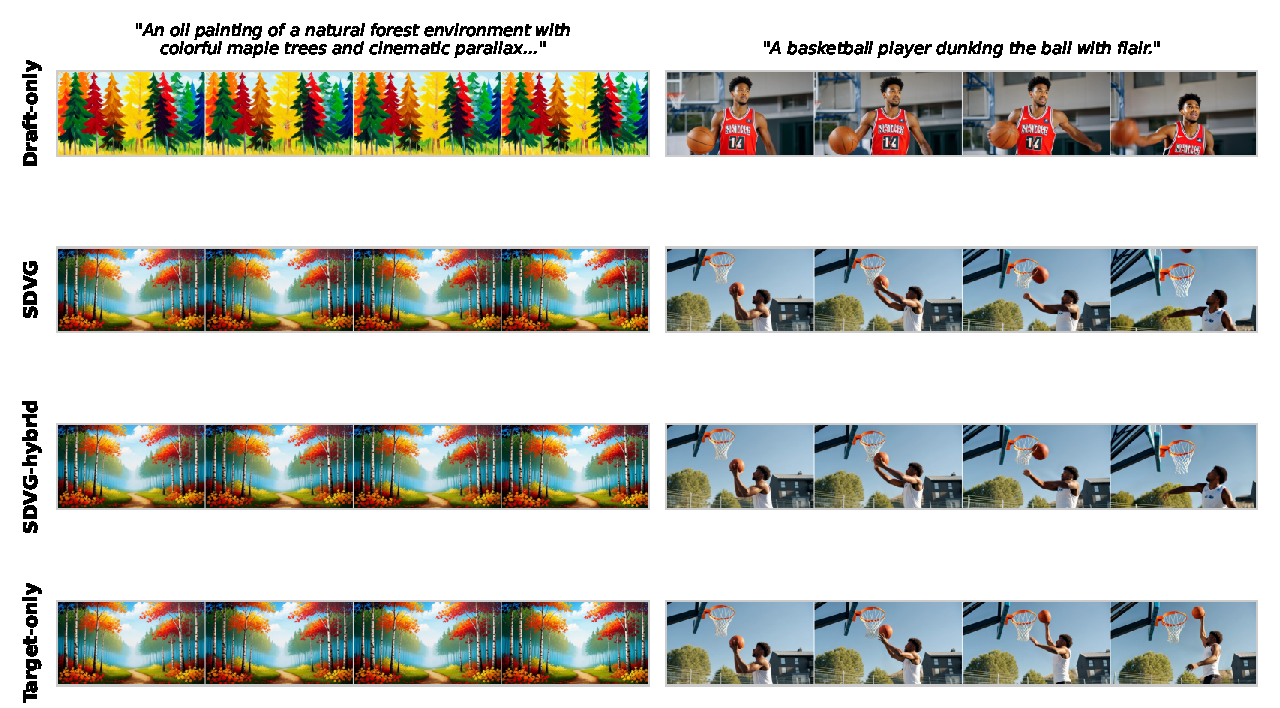
\includegraphics[width=\linewidth]{figures/appendix_qualitative_1}
  \caption{%
    Qualitative comparison on two further MovieGenVideoBench prompts.
    The draft's maple forest drifts in composition and saturation while
    both \texttt{SDVG} variants hold the target's palette, and on the
    basketball clip the draft loses the hoop and the player's limbs
    entirely.
  }
  \label{fig:app-qual-1}
\end{figure}

\begin{figure}[!htbp]
  \centering
  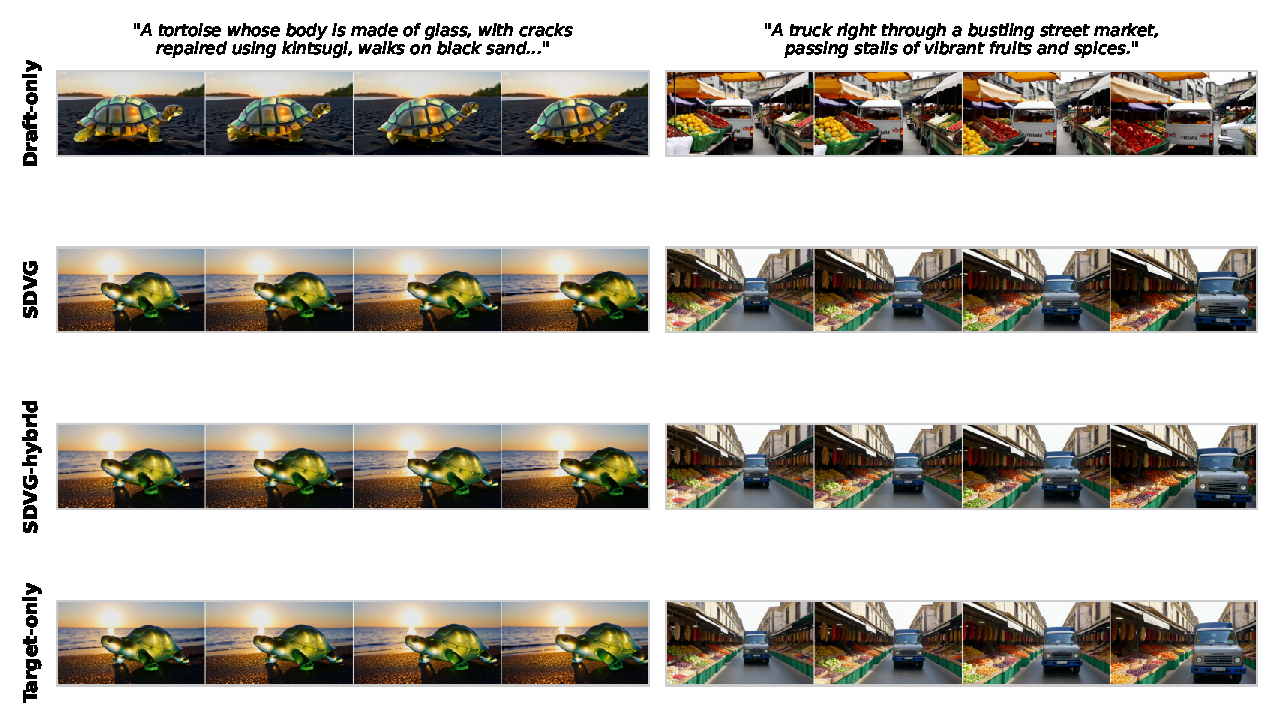
\includegraphics[width=\linewidth]{figures/appendix_qualitative_2}
  \caption{%
    Qualitative comparison on two further MovieGenVideoBench prompts.
    These two stress fine detail: the kintsugi cracks on the glass
    tortoise and the density of the market stalls both degrade in the
    draft and recover in the regenerated blocks.
  }
  \label{fig:app-qual-2}
\end{figure}

%%%%%%%%%%%%%%%%%%%%%%%%%%%%%%%%%%%%%%%%%%%%%%%%%%%%%%%%%%%%%%%%%%%%%%%%%%%%


\end{document}
